\documentclass[../uxoxo-main]{subfiles}
\begin{document}

\chapter{The Expressible and the Idealized UI}


\begingroup\itshape\small
\noindent
A user interface is modelled as a finite, typed, ordered tree of elements
carrying two transition systems --- an \emph{authoring} system that moves its
shape and a \emph{runtime} system that moves its state. We first make precise the
sense in which such a UI can express every valid state: \emph{generative
completeness}, from which a regular tree grammar, an instruction algebra, a
direct-manipulation editor, and decidability follow as four faces of one
reachable set. We then add a user. A \emph{preference} over the finite state
space is, by a representation theorem, a utility; its per-context maximizers form
an \emph{ideal policy} whose graph is a transversal of a context fibration, and
enforcing it is one more meet in a lattice of invariants --- a construction we
show is a meet-semilattice homomorphism into sub-transition-systems. A
\emph{usage model} learns this preference by Bayesian updating over a finite
hypothesis class from the trajectories of both transition systems; we prove
posterior consistency (the current weights converge to the ideal weights) under
realizability, identifiability, and exploration. A \emph{value-driven agent}
compiles the inferred ideal into a provably safe and reversible pre-pass, and we
prove that, with a confidence gate as the sole damping parameter, the closed loop
switches finitely often and converges. The idealized UI is therefore the
expressible UI under a learned invariant, cast preemptively --- no new power, one
new constraint.
\par\endgroup\medskip


% =====================================================================
\section{Preliminaries and standing assumptions}\label{iu:prelim}
\sectionnotation{the size bound $\mathsf B$ and the identity-isomorphism quotient; labelled transition system (LTS) and its induced sub-LTS $(\mathcal S,\to)\!\restriction_\phi$.}
% =====================================================================
We fix notation and two finiteness conventions used throughout.

A \textbf{labelled transition system} (LTS) is a pair $(\mathcal S,\to)$ with
$\to\,\subseteq\mathcal S\times\mathcal S$ (we suppress action labels when
irrelevant). For $\phi\subseteq\mathcal S$ the \textbf{induced sub-LTS} is
$(\mathcal S,\to)\!\restriction_\phi\;\coloneqq\;(\phi,\ \to\cap(\phi\times\phi))$:
keep the states in $\phi$ and the edges with both endpoints in $\phi$. We write
$\to^{*}$ for reflexive--transitive closure and call $(\mathcal S,\to)$
\textbf{strongly connected} if $s\to^{*}s'$ for all $s,s'$.

\begin{assumption}[Finite types and bounded size]\label{ass:finite}
The type alphabet $\Ttyp$ and the event alphabet $\Ev$ are finite, and every
type's state space $\St(\tau)$ is finite. We fix a \textbf{size bound}
$\mathsf{B}\in\Nat$ and consider only workspaces with $\lvert N\rvert\le\mathsf B$.
\end{assumption}

The size bound is what every \emph{finiteness} and \emph{optimization} claim
rests on; the purely \emph{structural} reachability results
(\cref{thm:univ}) hold without it. A bound is no loss of generality for a
deployed UI: a screen, a DOM, a scene graph are all finite.

\begin{assumption}[Identities are immaterial]\label{ass:iso}
Two workspaces are identified when related by a bijection of their node sets
preserving root, parent, child-order, and labels. All counting and optimization
are over isomorphism classes; ``the UI'' never depends on the names in $\II$.
\end{assumption}

This quotient is what makes the otherwise-unbounded identity domain $\II$
(over which key and reference constraints are not even regular) drop out of the
finite analysis: renaming nodes changes no observable.

% =====================================================================
\uxpart{Part A.\quad The expressible UI}
% =====================================================================

% ---------------------------------------------------------------------
\section{Workspaces and elements}\label{sec:workspaces}
\sectionnotation{workspace $W=(N,r,p,\chi,\ell)$, document $\Doc(W)$, descendant orders $\dle,\dleq,\dlplus$; well-formed set $\Tree$ and schema-valid $\Tree_\Sigma$; element $\delta=(\tau,A,S,E,\rho)$, state algebra $\St(\tau)$, region $\reg$; atomic vs.\ composite.}
% ---------------------------------------------------------------------
\begin{definition}[Workspace]\label{def:workspace}
A \textbf{workspace} is a tuple $W=(N,r,p,\chi,\ell)$ with $N$ a finite node set,
$r\in N$ a root, $p:N\pfun N$ a partial parent map, $\chi(n)$ a duplicate-free
ordering of $p^{-1}(n)$, and $\ell$ a labelling by elements (\cref{iu:elt}).
The \textbf{document} is the $r$-reachable part
$\Doc(W)\coloneqq\{n\in N: r\dleq n\}$, where $\dle$ is ``$=p(\cdot)$'' and
$\dleq$ its reflexive--transitive closure; nodes of $N\setminus\Doc(W)$ head
\textbf{detached fragments}. $W$ is \textbf{well-formed} when
\begin{enumerate}[label=\textbf{WF\arabic*.}, leftmargin=*, itemsep=1pt]
  \item $p$ is a partial function (at most one parent per node);
  \item $\chi(n)$ enumerates exactly $p^{-1}(n)$ without repetition;
  \item $\dlplus$ is irreflexive (acyclic; $(N,p)$ is a forest);
  \item $r\notin\Dom(p)$ and $\Doc(W)$ is the $r$-reachable set;
  \item $\ell$ is total and each label is well-typed (\cref{iu:elt}).
\end{enumerate}
$\Tree$ denotes the well-formed workspaces and, for a content model (schema)
$\Sigma$ fixing which types may parent which, $\Tree_\Sigma\coloneqq\{W\in\Tree:
\Sigma(W)\}$. The trivial schema $\Sigma\equiv\top$ gives the \emph{ideal} case.
\end{definition}

\begin{definition}[Element]\label{iu:elt}
A type $\tau\in\Ttyp$ denotes a finite state space $\St(\tau)$ built from atomic
state sets by product (\emph{concurrent}, $\lvert A\times B\rvert=\lvert A\rvert
\lvert B\rvert$), sum (\emph{exclusive}, $\lvert A+B\rvert=\lvert A\rvert+\lvert
B\rvert$), and least fixed point (\emph{nesting}, $\mu X.\,F(X)$). An
\textbf{element} is a tuple $\delta=(\tau,A,S,E,\rho)$: a type tag $\tau$; an
attribute record $A$ carrying at least a region $\reg(\delta)\subseteq\Real^{d}$;
the state space $S=\St(\tau)$; a handled alphabet $E\subseteq\Ev$; and a policy
$\rho$ comprising a partial \textbf{handler}
$\handle_\tau:S\times\Ev\pfun S$ with $\Dom(\handle_\tau)\subseteq S\times E$ (a
Mealy machine), a render contribution, and a \textbf{capability set}
$\kappa(n)\subseteq\{\mathsf{remove},\mathsf{reparent},\mathsf{reorder},
\mathsf{restyle},\mathsf{retype},\mathsf{addChild},\mathsf{rmChild}\}$. A node
with no children is an \textbf{atomic element} (a \emph{leaf}); an internal node
is a \textbf{composite element}.
\end{definition}

\begin{remark}[Composition is the tree]\label{rem:composition}
There is no separate ``composite'' primitive: a composite element \emph{is} an
internal node, and nesting \emph{is} composition. Geometric coherence
($\reg(n)\subseteq\reg(p(n))$ and disjoint sibling regions) makes hit-testing
(\cref{def:runtime}) total and deterministic.
\end{remark}

% ---------------------------------------------------------------------
\section{The authoring system}\label{sec:authoring}
\sectionnotation{the editor LTS $\Edit$; primitive operations $\Ops_\top=\{\mint,\attach,\detach,\delete,\relabel\}$ and derived $\move$; the authoring relation $\step{}$.}
% ---------------------------------------------------------------------
\begin{definition}[Editor]\label{def:editor}
An \textbf{editor} is an LTS $\Edit=(\mathcal S,\to)$, $\mathcal S\subseteq\Tree$,
whose steps are the \textbf{primitive operations}, each a partial function on
workspaces defined only when its result is again well-formed:
\begin{enumerate}[label=\textup{(\arabic*)}, leftmargin=*, itemsep=1pt]
  \item $\mint(\delta)\Rightarrow n$: add a fresh parentless node labelled
        $\delta$ (a singleton fragment); always defined.
  \item $\attach(n,q,k)$: when $n$ is a fragment root, $q$ lies outside $n$'s
        subtree, $0\le k\le\lvert\chi(q)\rvert$; set $p(n)=q$, insert $n$ at
        index $k$ of $\chi(q)$.
  \item $\detach(n)$: when $n\in\Dom(p)$, $n\ne r$; remove $n$ from $\chi(p(n))$
        and unset $p(n)$ (the subtree leaves with it).
  \item $\delete(n)$: when $n$ is a fragment root, $n\ne r$; remove $n$ and its
        subtree from $N$.
  \item $\relabel(n,\delta')$: set $\ell(n)=\delta'$ (refined into
        $\setType,\setAttr,\setStyle$ to touch one component).
\end{enumerate}
Write $\move(n,q,k)\coloneqq\detach(n);\attach(n,q,k)$ and
$\Ops_\top=\{\mint,\attach,\detach,\delete,\relabel\}$. A step is written
$W\step{}W'$; the relation $\step{}$ is the union of the primitive-operation
graphs.
\end{definition}

\begin{theorem}[Structural universality]\label{thm:univ}
From the seed $\Wempty$ (a lone root $r$), the set reachable under $\Ops_\top$ is
exactly $\Tree$, and $(\Tree,\step{})$ is strongly connected. Under
\cref{ass:finite} the same holds within $\Tree^{\le\mathsf B}$.
\end{theorem}

\begin{proof}
\emph{Soundness.} Each precondition returns the result to WF1--WF5: $\mint$ adds
an isolated labelled node; $\attach$'s no-cycle precondition preserves the forest
and updates $\chi$ consistently; $\detach$ splits off a subtree; $\delete$ drops
a tree; $\relabel$ touches only $\ell$. Hence $\step{}$ never leaves $\Tree$.

\emph{Completeness.} Fix a target $W^\star\in\Tree$. $\mint$ each node of
$W^\star$ with its target label; then visit the nodes of each tree of $W^\star$
in \emph{preorder} and $\attach$ every non-root beneath its target parent at its
target index. Preorder guarantees the parent is already present and rooted, so
each $\attach$ precondition holds; detached fragments are rebuilt the same way.
The result is $W^\star$. Every intermediate workspace has at most
$\lvert N(W^\star)\rvert$ nodes, so if $\lvert N(W^\star)\rvert\le\mathsf B$ the
build stays within $\Tree^{\le\mathsf B}$.

\emph{Strong connectivity.} From any $W$, repeatedly $\detach$ a leaf and
$\delete$ it (sizes only decrease), reaching $\Wempty$; composing the teardown of
$W$ with the build of $W'$ gives $W\step{}^{*}W'$. Sizes never exceed
$\max(\lvert N(W)\rvert,\lvert N(W')\rvert)$, so connectivity holds within
$\Tree^{\le\mathsf B}$ as well.
\end{proof}

\begin{proposition}[Primitivity --- no sealed compounds]\label{prop:primitive}
$\step{}^{*}$ is generated by single primitive steps: $W\step{}^{*}W'$ iff there
is a finite word $o_1\cdots o_m\in\Ops_\top^{*}$ carrying $W$ to $W'$.
Consequently every reachable transformation factors through the exposed
primitives, and any derived operation (e.g.\ $\move=\detach;\attach$) is
\emph{definitionally} such a word. There is no transformation reachable by some
compound $\mathsf{doXY}$ that its constituents $\mathsf{doX},\mathsf{doY}$ cannot
also achieve.
\end{proposition}

\begin{proof}
By \cref{def:editor} the one-step relation $\step{}$ is the union of the
primitive-operation graphs; $\step{}^{*}$ is its reflexive--transitive closure,
i.e.\ exactly the pairs joined by a finite word in $\Ops_\top$. A compound is by
definition a word in $\Ops_\top$, so its reachable set is contained in
$\step{}^{*}$, which by \cref{thm:univ} is all of $\Tree$ (resp.\
$\Tree^{\le\mathsf B}$). Hence no compound reaches outside the primitives'
closure.
\end{proof}

% ---------------------------------------------------------------------
\section{The runtime system, and finiteness}\label{sec:runtime}
\sectionnotation{runtime state $\varrho$ and its space $\mathrm{RT}(W)$; the no-dangling invariant $\Psi$; $\hit,\route,\handle$ and the runtime relation $\runstep{}$.}
% ---------------------------------------------------------------------
\begin{definition}[Runtime state]\label{def:runtime}
For $W$, a \textbf{runtime state} is
\[
  \varrho=(\sigma,\ \mathrm{focus},\ \mathrm{hover},\ \mathrm{capture},\
  \mathrm{drag},\ \mathrm{selection}).
\]
It carries a state map $\sigma:N\to\bigcup_n\St(\ell(n))$
with $\sigma(n)\in\St(\ell(n))$; pointer/keyboard globals
$\mathrm{focus},\mathrm{hover},\mathrm{capture}\in N\cup\{\bot\}$; a drag slot
$\mathrm{drag}\in(N\times\mathrm{payload})\cup\{\bot\}$; and a bounded
$\mathrm{selection}\subseteq N$. The space is $\mathrm{RT}(W)$. The
\textbf{no-dangling} invariant is
\begin{multline*}
  \Psi(W,\varrho)\coloniff
  \mathrm{focus},\mathrm{hover},\mathrm{capture}\in\Doc(W)\cup\{\bot\}\ \wedge\\
  \mathrm{drag}\in(\Doc(W)\!\times\!\mathrm{payload})\cup\{\bot\}\ \wedge\
  \mathrm{selection}\subseteq\Doc(W).
\end{multline*}
The \textbf{hit} of a point $x$ is the deepest node whose region contains $x$
(unique, by disjoint siblings); routing sends a pointer event to
$\mathrm{capture}$ or the hit, a key event to $\mathrm{focus}$. A
\textbf{runtime step} $\varrho\runstep{e}\varrho'$ (shape fixed) updates the
routed node's state by $\sigma(n)\mapsto\handle_{\tau(n)}(\sigma(n),e)$ when
$e\in E(n)$, with the guarded global updates, and preserves $\Psi$
automatically. Authoring steps that remove a node reset any global pointing into
it to $\bot$, re-establishing $\Psi$.
\end{definition}

\begin{theorem}[Finiteness and decidability of the per-workspace runtime]\label{thm:fin}
For fixed $W$ with each $\St(\ell(n))$ finite,
\[
  \mathrm{RT}(W)\ \cong\ \prod_{n\in N}\St(\ell(n))\ \times\
  (N\cup\{\bot\})^{3}\ \times\ \bigl((N\!\times\!\mathrm{payload})\cup\{\bot\}\bigr)
  \ \times\ \{U\subseteq N:\lvert U\rvert\le k\}
\]
is finite, so $(\mathrm{RT}(W),\runstep{})$ is a finite transition system and
reachability, equivalence, and LTL/CTL model-checking over it are decidable.
\end{theorem}

\begin{proof}
Each factor is finite ($N$ finite, $\St$ finite), so the product is finite;
$\runstep{}$ is a relation on a finite set, and the cited decision problems are
decidable for finite transition systems (standard).
\end{proof}

% ---------------------------------------------------------------------
\section{The UI-state space}\label{sec:uistate}
\sectionnotation{the UI state $s=(W,\varrho)$ and the (finite) UI-state space $\Ubd$.}
% ---------------------------------------------------------------------
\begin{definition}[UI state, UI-state space]\label{def:ustate}
A \textbf{UI state} is a pair $s=(W,\varrho)$ with $W\in\Tree_\Sigma$,
$\lvert N\rvert\le\mathsf B$, $\varrho\in\mathrm{RT}(W)$, and $\Psi(W,\varrho)$.
The \textbf{UI-state space} $\Ubd$ is the set of all such pairs, taken up to the
isomorphism of \cref{ass:iso}.
\end{definition}

\begin{proposition}[The state space is finite]\label{prop:Ufinite}
$\Ubd$ is finite and nonempty.
\end{proposition}

\begin{proof}
Nonempty: $(\Wempty,\varrho_0)\in\Ubd$. Finite: by \cref{ass:iso} a workspace of
size $\le\mathsf B$ is an isomorphism class of a finite rooted ordered forest on
$\le\mathsf B$ nodes labelled from the finite alphabet $\Ttyp$ (with finite
attribute records, themselves drawn from finite ranges under \cref{ass:finite});
there are finitely many such classes. For each, $\mathrm{RT}(W)$ is finite by
\cref{thm:fin}, and $\Psi$ cuts a subset. A finite union of finite sets is
finite.
\end{proof}

\begin{remark}[Validity is built in, not patched on]\label{rem:valid}
``Some configurations are invalid --- e.g.\ two radio buttons filled at once''
is handled at the level of the type algebra, not by an external filter. A radio
group of $n$ is the sum type $\sum_{n}1$, so ``exactly one filled'' holds by
construction: ``two filled'' is not a point of $\St(\tau)$. The general
discipline is to absorb impossible combinations into the type, or else carve
them out by a constraint or the schema $\Sigma$; the no-dangling invariant $\Psi$
removes the remaining invalid global states. $\Ubd$ is precisely what survives.
\end{remark}

% ---------------------------------------------------------------------
\section{Generative completeness and expressibility}\label{sec:gc}
\sectionnotation{generative completeness (structural $+$ behavioural) and \emph{expressibility}; initial state $s_0(\tau)$; the reachable set $\Reach(\Wempty,\step{}_\Sigma)$.}
% ---------------------------------------------------------------------
Write $s_0(\tau)\in\St(\tau)$ for a type's initial state and
$\Reach(\Wempty,\step{}_\Sigma)$ for the workspaces reachable from the seed under
the $\Sigma$-restricted primitives.

\begin{definition}[Generative completeness; expressibility]\label{def:gc}
A UI is \textbf{generatively complete} relative to $\Sigma$ when:
\emph{(a) structural} --- $(\Tree_\Sigma,\step{})$ is universal:
$\Reach(\Wempty,\step{}_\Sigma)=\Tree_\Sigma$ and the graph is strongly
connected; \emph{(b) behavioural} --- for each $\tau$, the runtime system
$(\St(\tau),\runstep{})$ generated by $\handle_\tau$ reaches all of $\St(\tau)$
from $s_0(\tau)$. It is \textbf{expressible} when, in addition, its authoring
moves are \emph{primitive} in the sense of \cref{prop:primitive}.
\end{definition}

Clause (a) is \cref{thm:univ}. Clause (b) is not automatic: a monotone handler
(a counter that only counts up) violates it. The repair is edit mode
(\cref{sec:edit}): a state no handler reaches at runtime can be \emph{set} as a
property.

\begin{remark}[The name]\label{rem:name}
\emph{Generative}, not \emph{Turing}: the runtime is deliberately finite-state
(\cref{thm:fin}), hence sub-Turing; completeness here is \emph{surjectivity of
the generators} (they reach every configuration), which is what keeps analysis
decidable. The word is apt because the property reads two ways that
\cref{sec:faces} shows coincide --- the operations \emph{generate} the reachable
set, the grammar \emph{generates} the language.
\end{remark}

% ---------------------------------------------------------------------
\section{Edit mode}\label{sec:edit}
\sectionnotation{the mode $m\in\{\modeUse,\modeEdit\}$; the capability set $\kappa(n)$; the mode escape.}
% ---------------------------------------------------------------------
\begin{definition}[Edit mode]\label{def:edit}
Augment the runtime state with a mode $m\in\{\modeUse,\modeEdit\}$. A gesture $g$
(with $e=\recognize(g)$, $n$ the routed node) dispatches on $m$: in $\modeUse$ it
is the runtime step $\sigma(n)\mapsto\handle_{\tau(n)}(\sigma(n),e)$; in
$\modeEdit$ it is an authoring operation on $\ell(n)$, permitted iff its kind
lies in $\kappa(n)$, with $\Psi$ re-established. The \textbf{escape} toggles $m$,
altering neither $W$ nor $\sigma$.
\end{definition}

\begin{proposition}[Carry-over]\label{prop:carry}
A use-mode state $(W,\sigma,\dots,\modeUse)$ and its escaped edit-mode state
$(W,\sigma,\dots,\modeEdit)$ share $(W,\sigma)$ and render identically. Any edit
issued in edit mode mutates that shared $W$; toggling back renders the mutated
$W$. Edit mode is uniform: every node is manipulable, gated by $\kappa(n)$ alone,
independently of $\handle_\tau$ --- an inert element ($\St(\tau)=1$) is still
editable.
\end{proposition}

\begin{proof}
Immediate from \cref{def:edit}: the toggle is identity on $(W,\sigma)$, and the
edit branch applies an authoring operation to the same $W$; capability gating
reads $\kappa(n)$ from $\rho$, which is defined for every node regardless of its
handler.
\end{proof}

% ---------------------------------------------------------------------
\section{The four faces of expressibility}\label{sec:faces}
\sectionnotation{the regular tree grammar $G_\Sigma$ with $L(G_\Sigma)$; the instruction algebra (State-monad actions); decidability of the finite system.}
% ---------------------------------------------------------------------
We exhibit the one reachable set $\Tree_\Sigma$ as a grammar, an instruction
algebra, a direct-manipulation editor, and a decidable object.

\paragraph{Face 1: the grammar.}
\begin{proposition}[Regular tree grammar]\label{prop:rtg}
The type algebra presents $\Ttyp$ as a regular tree grammar $G_\Sigma$: each
type is a nonterminal; a product $\St(\tau)=\prod_k\St(\tau_k)$ is a production
with right-hand side $\tau_1\cdots\tau_k$; a sum is a set of alternative
productions $\tau\to\tau_k$; a $\mu$ is a recursive nonterminal; the unit $1$ is
a leaf. The schema $\Sigma$ \emph{is} the production set, and $L(G_\Sigma)$ is a
regular tree language.
\end{proposition}

\begin{theorem}[Grammar $=$ reachable set]\label{thm:lang}
$L(G_\Sigma)=\Reach(\Wempty,\step{}_\Sigma)=\Tree_\Sigma$. Decorating each type
with its (finite) state, $\widehat{G}_\Sigma$ over
$\widehat\Ttyp=\bigsqcup_\tau(\{\tau\}\times\St(\tau))$ is still regular and
generates the states: $L(\widehat{G}_\Sigma)$ cut by $\Psi$ equals $\Ubd$.
\end{theorem}

\begin{proof}
($L(G_\Sigma)\subseteq\Tree_\Sigma$, $\supseteq$.) A leftmost $G_\Sigma$-derivation
of a tree $t$ expands nonterminals in preorder; reading each expansion as ``$\mint$
the child, $\attach$ it under the node just expanded, at the next index'' yields a
build sequence of \cref{thm:univ} producing exactly $t$, and the productions used
are the locally $\Sigma$-admissible ones, so $t\in\Tree_\Sigma$. Conversely the
preorder build sequence of \cref{thm:univ} for $W^\star\in\Tree_\Sigma$ reads off,
step by step, a $G_\Sigma$-derivation (mint $=$ choose a production for the child's
type; attach-in-preorder $=$ place it on the right-hand side), so
$W^\star\in L(G_\Sigma)$. The middle equality is \cref{thm:univ}. Finiteness of
each $\St(\tau)$ makes $\widehat{G}_\Sigma$ a finite decoration, hence regular;
its trees are the labelled-with-state workspaces, and intersecting with the
(non-regular but invariant) $\Psi$ gives the valid states $\Ubd$.
\end{proof}

\paragraph{Face 2: the instruction algebra (quantified change).}
An \textbf{instruction} is a named operator with a binding from a finite
parameter profile to values; its meaning is a function
$f:B_{\mathrm{valid}}\to T(R)$ into an effect monad $T$, total on valid bindings.
For the editor, $T$ is the State monad over workspaces and each primitive of
\cref{def:editor} is one instruction. A \textbf{program} $c_1;\dots;c_m$ denotes
the composite $f_{c_m}\bullet\cdots\bullet f_{c_1}$ in $T$.

\begin{proposition}[State and change are quantified]\label{prop:instr}
Each $s\in\Ubd$ is a term of the instruction algebra (its build program); each
single state change is an instruction; each multi-step change is a program ---
the composite of the corresponding State-monad actions. The build map from terms
to workspaces is onto $\Tree_\Sigma$.
\end{proposition}

\begin{proof}
The instruction constructors freely generate a term algebra; assigning each its
State-monad action makes workspaces an algebra and the build map the unique
homomorphism. Ontoness is \cref{thm:univ} (every workspace is some build
program's value); a state change is the action of the instruction effecting it;
sequencing is composition in $T$.
\end{proof}

\paragraph{Face 3: direct manipulation.}
Equip the document with a render $\Render:\Tree\to\View$ and a lift $\Lift$
sending a gesture to an operation, with the WYSIWYG square
$\Render(W\cdot\Lift(W,g))=g\cdot\Render(W)$.

\begin{theorem}[Direct-manipulation completeness]\label{thm:dm}
Assume $\Render$ injective on editing-relevant structure and $\Lift$ total over
the gestures needed to reach any view. Then edit-mode gestures realize every
authoring operation, so $\Reach_{\modeEdit}=\Tree_\Sigma$: every $\Sigma$-valid
UI is buildable by direct manipulation. Restricting permitted operations by
$\kappa$ cuts this to the corresponding invariant subspace.
\end{theorem}

\begin{proof}
Under the hypotheses $\Lift$ surjects the gestures onto $\Ops_\top$ on each view,
and $\Render$ being injective on editing-relevant structure means distinct
editable states have distinct views, so a gesture sequence realizing a build
sequence of \cref{thm:univ} exists; transporting \cref{thm:univ} across $\Render$
gives reachability of every view. Capability gating removes exactly the gestures
whose lifted operation violates the relevant invariant.
\end{proof}

\paragraph{Face 4: decidability.}
\begin{corollary}[Decidability]\label{cor:dec}
$\Ubd$ is finite (\cref{prop:Ufinite}) and the joint authoring/runtime relation
on it is a finite transition system, so reachability, equivalence, and LTL/CTL
queries over the UI are decidable.
\end{corollary}

\begin{proof}
Finiteness is \cref{prop:Ufinite}; both relations are relations on a finite set;
apply \cref{thm:fin}'s decidability to the joint system.
\end{proof}

\begin{theorem}[Summary: the four faces]\label{thm:faces}
For an expressible UI the following describe one set, $\Tree_\Sigma$ (resp.\
its decorated form $\Ubd$): the grammar $L(G_\Sigma)$ (\cref{thm:lang}); the
image of the build homomorphism of the instruction algebra
(\cref{prop:instr}); the direct-manipulation reachable set $\Reach_{\modeEdit}$
(\cref{thm:dm}); and a finite, decidable transition system (\cref{cor:dec}).
None enlarges expressibility; each re-presents it.
\end{theorem}

\begin{proof}
Each clause is the cited result; their common right-hand side is $\Tree_\Sigma$
(states $\Ubd$) by \cref{thm:univ}.
\end{proof}

% =====================================================================
\uxpart{Part B.\quad Preference and the ideal}
% =====================================================================

% ---------------------------------------------------------------------
\section{Contexts as a fibration}\label{sec:ctx}
\sectionnotation{the context projection $\proj:\Ubd\twoheadrightarrow\Ctx$ and its fibers $\Ufib{x}$.}
% ---------------------------------------------------------------------
A preference need not rank states absolutely; it ranks them \emph{given} what is
fixed --- the content the user is working with, the task, the device. We model
``what is fixed'' as a projection and optimize within its fibers.

\begin{definition}[Context fibration]\label{def:ctx}
A \textbf{context projection} is a surjection $\proj:\Ubd\twoheadrightarrow\Ctx$
onto a finite set of \textbf{contexts}, with $\proj(s)$ the fixed part of $s$.
Its \textbf{fibers} are $\Ufib{x}\coloneqq\proj^{-1}(x)$, the states agreeing on
the fixed part. (Choosing $\proj$ to forget exactly the user-mutable
presentation makes the fibers the ``free'' part the system may personalize.)
\end{definition}

\begin{remark}[Two readings of context]\label{rem:ctx}
Reading $\proj$ as an \emph{endogenous} feature of the state (the document
content) makes the fibration intrinsic and the ideal a transversal
(\cref{sec:ideal}). Reading context as an \emph{exogenous} signal (time, locale)
is the special case where $\proj$ factors through that signal; then a change of
context is an event that moves the user to a new fiber, handled by the loop of
\cref{sec:loop}. We develop the endogenous reading; the exogenous one is a
corollary via the loop.
\end{remark}

% ---------------------------------------------------------------------
\section{Preference and its utility representation}\label{sec:pref}
\sectionnotation{the preference structure $\{\succeq_x\}_{x}$ (a total preorder per fiber) and the utility $U_\uu$.}
% ---------------------------------------------------------------------
\begin{definition}[Preference structure]\label{def:pref}
A \textbf{preference structure} for user $\uu$ is a family
$\{\succeq_x\}_{x\in\Ctx}$ where each $\succeq_x$ is a \emph{total preorder}
(reflexive, transitive, total) on the fiber $\Ufib{x}$. Write $\succ_x$ and
$\sim_x$ for its strict and indifference parts.
\end{definition}

The content of the coherence hypothesis is exactly these axioms; the utility is
then not an assumption but a theorem.

\begin{theorem}[Utility representation]\label{thm:rep}
For each total preorder $\succeq_x$ on the finite set $\Ufib{x}$ there is a utility
$U_\uu(x,\cdot):\Ufib{x}\to\Real$ with
\[
  s\succeq_x s'\iff U_\uu(x,s)\ge U_\uu(x,s')\qquad(s,s'\in\Ufib{x}).
\]
$U_\uu$ is unique up to a per-fiber strictly increasing transformation.
\end{theorem}

\begin{proof}
Let $\sim_x$ be the indifference relation ($s\sim_x s'$ iff $s\succeq_x s'$ and
$s'\succeq_x s$); by reflexivity, transitivity, and totality it is an
equivalence, and $\succeq_x$ descends to a total \emph{order} (antisymmetric
total preorder) on the finite quotient $\Ufib{x}/\!\sim_x$. A finite totally
ordered set $\{[s_1]\prec\cdots\prec[s_m]\}$ embeds order-preservingly into
$\Real$ by $[s_i]\mapsto i$. Set $U_\uu(x,s)\coloneqq i$ for $s\in[s_i]$. Then
$s\succeq_x s'$ iff $[s]\succeq[s']$ iff their indices compare, iff
$U_\uu(x,s)\ge U_\uu(x,s')$. Any strictly increasing reparametrization of the
indices represents the same order, and any representing utility induces the same
order, giving uniqueness up to such a transformation.
\end{proof}

\begin{assumption}[Coherence]\label{ass:coh}
$\uu$'s preference is a preference structure (\cref{def:pref}) and is
\emph{stationary} over the horizon considered. Equivalently, by \cref{thm:rep}, a
fixed utility $U_\uu:\{(x,s):s\in\Ufib{x}\}\to\Real$ exists.
\end{assumption}

Coherence is a genuine restriction --- real preferences can be intransitive,
fiber-entangled, or drifting. It is the analogue here of the
$\Render$-injectivity hypothesis of \cref{thm:dm}: stated, not assumed away.

% ---------------------------------------------------------------------
\section{The ideal policy and the optimal transversal}\label{sec:ideal}
\sectionnotation{the ideal policy $\pi^\star_\uu$ and the optimal transversal $\Uopt=\img(\pi^\star_\uu)$.}
% ---------------------------------------------------------------------
\begin{definition}[Ideal policy; optimal state space]\label{def:idealpolicy}
Under \cref{ass:coh}, an \textbf{ideal policy} is any
$\pi^\star_\uu:\Ctx\to\Ubd$ with
\[
  \pi^\star_\uu(x)\in\argmax_{s\in\Ufib{x}}U_\uu(x,s)\qquad(\text{ties broken by a
  fixed order on }\Ubd).
\]
Its graph $\Uopt\coloneqq\img(\pi^\star_\uu)=\{\pi^\star_\uu(x):x\in\Ctx\}$
is the \textbf{optimal state space}.
\end{definition}

\begin{proposition}[The ideal exists, and is a transversal]\label{prop:idealexists}
$\pi^\star_\uu$ exists, $\proj(\pi^\star_\uu(x))=x$, and $\Uopt$ meets each
fiber in exactly one state: it is a \emph{transversal} of the fibration
$\proj$, with $\lvert\Uopt\rvert=\lvert\Ctx\rvert$.
\end{proposition}

\begin{proof}
Each fiber $\Ufib{x}$ is finite (a subset of the finite $\Ubd$,
\cref{prop:Ufinite}) and nonempty (since $\proj$ is onto), so
$U_\uu(x,\cdot)$ attains its maximum on it and the (tie-broken) maximizer
$\pi^\star_\uu(x)$ is a well-defined element \emph{of $\Ufib{x}$}; hence
$\proj(\pi^\star_\uu(x))=x$. Thus $\pi^\star_\uu(x)$ is the unique member of
$\Uopt$ in fiber $x$, and distinct contexts give distinct fibers, so
$\lvert\Uopt\rvert=\lvert\Ctx\rvert$.
\end{proof}

That ``an ideal state exists'' is thus \emph{finiteness}
(\cref{prop:Ufinite}), not idealization; coherence (\cref{ass:coh}) only makes
the ideal \emph{well-defined}.

% ---------------------------------------------------------------------
\section{The invariant lattice, precisely}\label{sec:lattice}
\sectionnotation{invariants as the lattice $2^{\Ubd}$; the induced sub-LTS $\mathsf S(\phi)$ and the meet-semilattice homomorphism.}
% ---------------------------------------------------------------------
Schema, protection, no-dangling, and (below) preference are all invariants of
one lattice; restricting the editor by any of them is taking the induced sub-LTS.
We make the ``lattice'' exact.

\begin{definition}[Invariants and induced subsystems]\label{def:invlat}
An \textbf{invariant} is a predicate $\phi$ on $\Ubd$, identified with the set
$\llbracket\phi\rrbracket\subseteq\Ubd$. Invariants are ordered by implication
$\phi\le\psi\iff\llbracket\phi\rrbracket\subseteq\llbracket\psi\rrbracket$; this
is the complete lattice $(2^{\Ubd},\subseteq)$ with meet $\wedge=\cap$, join
$\vee=\cup$, top $\top=\Ubd$. For an LTS $(\Ubd,\to)$ let
$\mathsf S(\phi)\coloneqq(\Ubd,\to)\!\restriction_{\llbracket\phi\rrbracket}$ be
the induced sub-LTS; order sub-LTSs by componentwise inclusion of states and
edges, with meet $\sqcap$ given by intersection of state sets and edge sets.
\end{definition}

\begin{theorem}[Restriction is a meet-semilattice homomorphism]\label{thm:latticehom}
$\mathsf S$ is monotone and preserves arbitrary meets:
$\mathsf S\!\bigl(\bigwedge_i\phi_i\bigr)=\bigsqcap_i\mathsf S(\phi_i)$. In
particular the editor constrained by two invariants is the meet of the two
restricted editors. $\mathsf S$ need not preserve joins.
\end{theorem}

\begin{proof}
\emph{Monotone:} if $\llbracket\phi\rrbracket\subseteq\llbracket\psi\rrbracket$
then $\llbracket\phi\rrbracket$-states are $\llbracket\psi\rrbracket$-states and
edges within $\llbracket\phi\rrbracket$ are edges within
$\llbracket\psi\rrbracket$, so $\mathsf S(\phi)$ is a sub-LTS of $\mathsf
S(\psi)$. \emph{Meets:} write $P_i=\llbracket\phi_i\rrbracket$ and $P=\bigcap_i
P_i$. The states of $\mathsf S(\bigwedge_i\phi_i)$ are $P$; its edges are
$\to\cap(P\times P)$. The states of $\bigsqcap_i\mathsf S(\phi_i)$ are
$\bigcap_iP_i=P$; its edges are $\bigcap_i\bigl(\to\cap(P_i\times P_i)\bigr)=
\to\cap\bigcap_i(P_i\times P_i)=\to\cap(P\times P)$, using
$\bigcap_i(P_i\times P_i)=(\bigcap_iP_i)\times(\bigcap_iP_i)$ (a pair lies in
every $P_i\times P_i$ iff both coordinates lie in every $P_i$). The two
subsystems coincide. \emph{Joins fail:} for $P_1\ne P_2$ an edge between a
$P_1$-only and a $P_2$-only state lies in $\to\cap((P_1\cup P_2)^{2})$ but in
neither $\to\cap(P_i^{2})$, so
$\mathsf S(\phi_1\vee\phi_2)\ne\mathsf S(\phi_1)\sqcup\mathsf S(\phi_2)$ in
general.
\end{proof}

\begin{example}[The shipped invariants]\label{ex:invariants}
The schema $\Sigma$, the protection invariant $\Phi^{\theta}_{P}$ (a fixed set of
nodes kept in the document with frozen types), and the no-dangling $\Psi$ are
invariants; the editor one ships is the meet $\Sigma\wedge\Psi\wedge\Phi^\theta_P$
and its state space is $\mathsf S$ of that meet. The ideal editor is the top
$\top$.
\end{example}

% ---------------------------------------------------------------------
\section{Personalization as a learned invariant}\label{sec:phiu}
\sectionnotation{the preference invariant $\Phiu$ and the personalized configuration.}
% ---------------------------------------------------------------------
\begin{definition}[Preference invariant; personalized configuration]\label{def:phiu}
The \textbf{preference invariant} pins a state to the optimum for its own
context:
\[
  \Phiu(s)\coloniff s=\pi^\star_\uu(\proj(s)).
\]
The \textbf{personalized configuration} is $\mathsf S(\Phiu)$ on
$\Sigma\wedge\Psi\wedge\Phi^\theta_P$, i.e.\ the induced subsystem of the meet
$\Sigma\wedge\Psi\wedge\Phi^\theta_P\wedge\Phiu$.
\end{definition}

\begin{proposition}[The personalized state space is the optimal transversal]\label{prop:phiu}
$\llbracket\Phiu\rrbracket=\Uopt$, and on it every realized state is a
$U_\uu$-maximizer for its context:
$U_\uu(\proj(s),s)=\max_{s'\in\Ufib{\proj(s)}}U_\uu(\proj(s),s')$ for all
$s\in\Uopt$. By \cref{thm:latticehom} the personalized configuration is one
more meet in the lattice of \cref{ex:invariants}; it is a restriction and need
not be strongly connected.
\end{proposition}

\begin{proof}
$s\in\llbracket\Phiu\rrbracket$ iff $s=\pi^\star_\uu(\proj(s))$, i.e.\ $s$ is the
fiber-$\proj(s)$ optimum; by \cref{prop:idealexists} these are exactly the
transversal points $\Uopt$, on which the maximizer property holds by
\cref{def:idealpolicy}. The meet statement is \cref{thm:latticehom} applied to
$\Sigma\wedge\Psi\wedge\Phi^\theta_P\wedge\Phiu$. Strong connectivity is not
claimed: a transversal can have any internal edge structure, including none.
\end{proof}

What \emph{is} guaranteed --- and is all the agent needs --- is that the optimum
is reachable \emph{from default} in the unrestricted editor, by strong
connectivity (\cref{thm:univ}).

\begin{center}
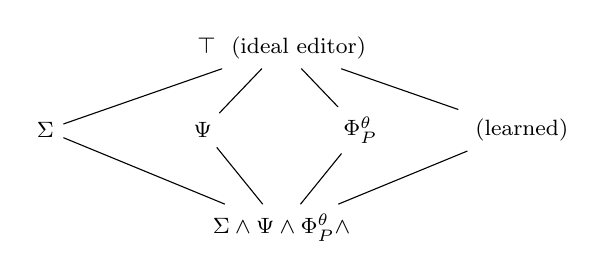
\begin{tikzpicture}[every node/.style={font=\footnotesize}, line cap=round,
                    yscale=0.95]
  \node (top) at (0,2)      {$\top$\ \ (ideal editor)};
  \node (sig) at (-3,0.9)   {$\Sigma$};
  \node (psi) at (-1,0.9)   {$\Psi$};
  \node (phi) at (1,0.9)    {$\Phi^{\theta}_{P}$};
  \node (phu) at (3,0.9)    {$\Phiu$ (learned)};
  \node (bot) at (0,-0.4)   {$\Sigma\wedge\Psi\wedge\Phi^{\theta}_{P}\wedge\Phiu$};
  \draw (top)--(sig); \draw (top)--(psi); \draw (top)--(phi); \draw (top)--(phu);
  \draw (sig)--(bot); \draw (psi)--(bot); \draw (phi)--(bot); \draw (phu)--(bot);
\end{tikzpicture}
\end{center}

% =====================================================================
\uxpart{Part C.\quad Learning the ideal}
% =====================================================================

% ---------------------------------------------------------------------
\section{The behavioural observation model}\label{sec:obs}
\sectionnotation{actions $a$ (interactions and edits); the Boltzmann/Gibbs behavioural law $\law_\theta(a\mid s)$ with rationality $\beta$.}
% ---------------------------------------------------------------------
The data are not annotations but the user's own steps in the two transition
systems. An action reveals a noisy preference for where the user steered the UI.

\begin{definition}[Action, behavioural law]\label{def:obs}
At a UI state $s$ (context $x=\proj(s)$) the user takes an \textbf{action} $a$ ---
a $\kappa$-permitted instruction (an \emph{explicit modification}, a step of
$\step{}$) or a runtime event (a \emph{normal interaction}, a step of
$\runstep{}$) --- reaching $s'=a\cdot s$. Let $\mathcal A(s)$ be the finite set of
available actions. Given a candidate utility $U_\theta$, the
\textbf{behavioural law} is the Gibbs (Boltzmann-rational) choice
\[
  \law_\theta(a\mid s)\;=\;
  \frac{\exp\!\bigl(\beta\,U_\theta(\proj(a\cdot s),\,a\cdot s)\bigr)}
       {\displaystyle\sum_{a'\in\mathcal A(s)}\exp\!\bigl(\beta\,U_\theta(\proj(a'\cdot s),\,a'\cdot s)\bigr)},
  \qquad\beta>0,
\]
so higher-utility destinations are more probable, deterministically optimal as
$\beta\to\infty$. The likelihood of a trace $\langle(s_i,a_i)\rangle_{i=1}^{t}$
is $\prod_{i=1}^{t}\law_\theta(a_i\mid s_i)$ (Markov).
\end{definition}

Both transition systems feed one likelihood: an edit and an interaction are both
actions, differing only in which destinations they make available. This is the
precise sense in which the model ``updates on both normal interactions and
explicit modifications.''

% ---------------------------------------------------------------------
\section{The usage model and the Bayes update}\label{sec:bayes}
\sectionnotation{the finite hypothesis class $\Theta$ and prior $\mu_0$; the posterior (usage model) $\mu_t$, the Bayes operator $\learn$, and the MAP estimate $\hat\theta_t$.}
% ---------------------------------------------------------------------
\begin{definition}[Hypothesis class, usage model, learning]\label{def:usage}
Fix a finite \textbf{hypothesis class} $\Theta$ of candidate utilities (the
``weights''), and a prior $\mu_0\in\Delta(\Theta)$. The \textbf{usage model} at
time $t$ is the posterior $\mu_t\in\Delta(\Theta)$. \textbf{Learning} is the
Bayes operator
\[
  \mu_{t+1}\;=\;\learn(\mu_t,(s_t,a_t))\;\propto\;
  \mu_t(\cdot)\,\law_{(\cdot)}(a_t\mid s_t),
\]
a function of interaction history with \emph{no} side effect on any workspace
(the descriptive ``wall''). The \textbf{current weights} are $\mu_t$ (or its mode
$\hat\theta_t=\argmax_\theta\mu_t(\theta)$).
\end{definition}

A finite $\Theta$ keeps the update exact and every downstream quantity
computable; a continuous $\Theta$ is the practical case but is not needed for the
results below.

\begin{definition}[Ideal weights; alignment]\label{def:align}
The \textbf{ideal weights} $\theta^\star\in\Theta$ are those representing the true
preference (\cref{ass:real}). The current and ideal weights are two distinct
points of $\Theta$ --- the realized estimate and the oracle target --- related by
the \textbf{alignment operator} $\Lambda=\lim_{t}\learn(\,\cdot\,;\text{history}_{\le t})$,
the Bayes update iterated to its limit.
\end{definition}

% ---------------------------------------------------------------------
\section{Consistency: the current weights reach the ideal}\label{sec:consistency}
\sectionnotation{realizability and the ideal weights $\theta^\star$; the alignment operator $\Lambda$; the divergence $\KL$.}
% ---------------------------------------------------------------------
\begin{assumption}[Realizability]\label{ass:real}
The true behavioural law is $\law_{\theta^\star}$ for some
$\theta^\star\in\Theta$, and $\mu_0(\theta^\star)>0$.
\end{assumption}

\begin{assumption}[Identifiability and exploration]\label{ass:ident}
For every $\theta\ne\theta^\star$ there is a state $s$ reachable infinitely often
under the data-generating process with
$\law_\theta(\cdot\mid s)\ne\law_{\theta^\star}(\cdot\mid s)$; and at each such
$s$ the realized actions are drawn from $\law_{\theta^\star}(\cdot\mid s)$
independently across visits. (Distinct utilities are behaviourally
distinguishable, and the distinguishing situations recur.)
\end{assumption}

\begin{theorem}[Posterior consistency / alignment]\label{thm:consistency}
Under \cref{ass:real,ass:ident}, $\mu_t(\theta^\star)\to1$ almost surely; hence
$\hat\theta_t=\theta^\star$ for all large $t$, and the alignment operator
$\Lambda$ carries any admissible prior to the point mass $\delta_{\theta^\star}$.
\end{theorem}

\begin{proof}
Fix $\theta\ne\theta^\star$. From the Bayes recursion the posterior odds factor:
\[
  \frac{\mu_t(\theta)}{\mu_t(\theta^\star)}
  =\frac{\mu_0(\theta)}{\mu_0(\theta^\star)}\,
   \prod_{i=1}^{t}\frac{\law_\theta(a_i\mid s_i)}{\law_{\theta^\star}(a_i\mid s_i)},
\]
so $\log\frac{\mu_t(\theta)}{\mu_t(\theta^\star)}
=\log\frac{\mu_0(\theta)}{\mu_0(\theta^\star)}+\sum_{i=1}^{t}Z_i$ with
$Z_i=\log\frac{\law_\theta(a_i\mid s_i)}{\law_{\theta^\star}(a_i\mid s_i)}$.
Group the steps by the state visited. At any state $s$ with
$\law_\theta(\cdot\mid s)\ne\law_{\theta^\star}(\cdot\mid s)$, the per-visit
conditional expectation is
$\E_{\theta^\star}[Z\mid s]=-\KL\!\bigl(\law_{\theta^\star}(\cdot\mid s)\,\Vert\,
\law_\theta(\cdot\mid s)\bigr)<0$, strictly, since the laws differ and KL
vanishes only for identical laws. By \cref{ass:ident} at least one such $s$ is
visited infinitely often with i.i.d.\ draws, so along that subsequence the strong
law of large numbers makes the running average of $Z$ converge to a strictly
negative constant; the contributions of states where the laws agree are
identically zero. Hence $\sum_{i\le t}Z_i\to-\infty$ a.s., so the odds
$\frac{\mu_t(\theta)}{\mu_t(\theta^\star)}\to0$, i.e.\ $\mu_t(\theta)\to0$.
As $\Theta$ is finite and the masses sum to one, $\mu_t(\theta^\star)\to1$ a.s.
Consequently, for large $t$, $\mu_t(\theta^\star)>\mu_t(\theta)$ for every
$\theta\ne\theta^\star$, so $\hat\theta_t=\theta^\star$; and $\Lambda$, the limit
of the update, sends the prior to $\delta_{\theta^\star}$.
\end{proof}

\begin{remark}[Misspecification]\label{rem:misspec}
If $\theta^\star\notin\Theta$ (no candidate is exactly right), the same odds
computation, with $\E[Z\mid s]=\KL(\law_{\mathrm{true}}\Vert\law_{\theta'})-
\KL(\law_{\mathrm{true}}\Vert\law_\theta)$, shows the posterior concentrates on
the information projection
$\theta^\dagger=\argmin_{\theta\in\Theta}\sum_{s}w(s)\,
\KL\!\bigl(\law_{\mathrm{true}}(\cdot\mid s)\Vert\law_\theta(\cdot\mid s)\bigr)$
($w$ the visit frequencies): the best-in-class hypothesis. The conclusions below
then hold for the best achievable policy rather than the true one.
\end{remark}

% ---------------------------------------------------------------------
\section{The predictive law and the MAP policy}\label{sec:map}
\sectionnotation{the fiber Gibbs law $\Glaw_\theta(s\mid x)$ and the MAP policy $\hat\pi_\theta$.}
% ---------------------------------------------------------------------
The agent needs not the next action but the \emph{destination}: the best state in
the current fiber. Utility and probability are one object here.

\begin{definition}[Fiber Gibbs law; MAP policy]\label{def:map}
For $\theta$ and context $x$, the \textbf{fiber Gibbs law}
$\Glaw_\theta(s\mid x)\propto\exp(\beta\,U_\theta(x,s))$ on $\Ufib{x}$ is the
predictive law over which state should hold. Its \textbf{mode} is the
\textbf{MAP policy} $\hat\pi_\theta(x)=\argmax_{s\in\Ufib{x}}\Glaw_\theta(s\mid x)$.
\end{definition}

\begin{proposition}[Mode $=$ utility-argmax $=$ ideal at $\theta^\star$]\label{prop:map}
For every $\beta>0$, $\hat\pi_\theta(x)=\argmax_{s\in\Ufib{x}}U_\theta(x,s)$. Hence
under \cref{ass:coh,ass:real}, $\hat\pi_{\theta^\star}=\pi^\star_\uu$, and by
\cref{thm:consistency} $\hat\pi_{\hat\theta_t}\to\pi^\star_\uu$. The ``highest
probability'' state of \cref{def:map} and the ``ideal'' state of
\cref{def:idealpolicy} are the same object; the argmax of either is the ideal.
\end{proposition}

\begin{proof}
$\exp(\beta\,\cdot)$ is strictly increasing, so it preserves the maximizer:
$\argmax_s\Glaw_\theta(s\mid x)=\argmax_s U_\theta(x,s)$. At $\theta^\star$,
$U_{\theta^\star}=U_\uu$ (\cref{ass:real} with \cref{thm:rep}), so the mode is
$\pi^\star_\uu(x)$ by \cref{def:idealpolicy}. Convergence
$\hat\theta_t\to\theta^\star$ (\cref{thm:consistency}) gives
$\hat\pi_{\hat\theta_t}=\hat\pi_{\theta^\star}=\pi^\star_\uu$ for large $t$.
\end{proof}

% =====================================================================
\uxpart{Part D.\quad The agent and the loop}
% =====================================================================

% ---------------------------------------------------------------------
\section{The value-driven agent}\label{sec:agent}
\sectionnotation{the glamour and grimoire; the value-driven agent $F$ and its value function $U$; the idealized UI tuple.}
% ---------------------------------------------------------------------
\begin{definition}[Glamour, grimoire, the agent $F$]\label{def:agent}
A \textbf{glamour} is a typed conditional rewrite $(\text{guard},\text{action})$
with guard a predicate on $(\text{node},\text{context})$ and action a
$\kappa$-permitted instruction; a \textbf{grimoire} is a finite set of glamours.
The \textbf{agent} $F$ is parameterized by a value function $U$ (its ``values'').
From $U$ it compiles the grimoire whose glamour for context $x$ has guard
$\proj=x$ and action a $\kappa$-permitted program driving the default workspace
$T_0$ toward $\hat\pi(x)$ (\cref{def:map}); as a \textbf{pre-pass} --- before the
runtime layer takes the stage --- $F$ emits that program and applies it, yielding
the personalized $\langle T_F,\varrho_F\rangle$. $F$ does not learn.
\end{definition}

\begin{theorem}[Safety, reachability, reversibility]\label{thm:agent}
Under \cref{ass:coh} (so $\hat\pi$ is defined) and expressibility, the agent $F$
of \cref{def:agent} satisfies:
\begin{enumerate}[label=\textup{(\roman*)}, leftmargin=*, itemsep=1pt]
  \item \emph{(reachability)} the target $\hat\pi(\proj(T_0))$ is reachable from
        $T_0$, so $F$'s program exists;
  \item \emph{(closure / safety)} $\langle T_F,\varrho_F\rangle\in\Tree_\Sigma$
        with $\Sigma$ and $\Psi$ intact;
  \item \emph{(reversibility)} $F$'s effect is undoable and reset-to-default is
        reachable from any personalized state.
\end{enumerate}
\end{theorem}

\begin{proof}
(i) By \cref{prop:idealexists} the target is a state of $\Ubd$; by
\cref{thm:univ} (strong connectivity) a sequence of primitives carries $T_0$ to
it, and restricting to $\kappa$-permitted primitives still suffices because the
target satisfies the capability constraints by construction. (ii) Each
$\kappa$-permitted instruction preserves $\Sigma$ (it is a step of the restricted
editor, the induced subsystem $\mathsf S(\Sigma\wedge\dots)$ of
\cref{thm:latticehom}) and preserves $\Psi$ (removals re-establish it,
\cref{def:runtime}); invariant preservation composes because the meet of
invariants is itself an invariant (\cref{thm:latticehom}), so the whole program
keeps the output in $\mathsf S(\Sigma\wedge\Psi\wedge\dots)\subseteq\Tree_\Sigma$.
(iii) The effect is a program of primitives and $(\Tree,\step{})$ is strongly
connected (\cref{thm:univ}), so $\Wempty$ --- and any prior state --- is reachable
from the personalized state; undo is the reverse path.
\end{proof}

\begin{definition}[The idealized UI]\label{def:idealui}
For user $\uu$ the \textbf{idealized UI} is the tuple
$\mathcal I_\uu=(U_\uu,\proj,\Theta,\learn,\theta^\star,\pi^\star_\uu,\Phiu,F)$:
an expressible UI (Part~A) with a coherent utility over a context fibration
(\cref{ass:coh,def:ctx}), a usage model and its Bayes update
(\cref{def:usage}), aligned current/ideal weights (\cref{def:align,thm:consistency}),
the induced ideal policy (\cref{def:idealpolicy}), the learned invariant carving
the optimal transversal (\cref{def:phiu}), and the value-driven agent that
preemptively casts it (\cref{def:agent,thm:agent}).
\end{definition}

% ---------------------------------------------------------------------
\section{The closed loop and non-thrashing}\label{sec:loop}
\sectionnotation{the closed loop with confidence gate $\epsilon$; the installed hypothesis and the non-thrashing argument.}
% ---------------------------------------------------------------------
The organs close a loop: $F$ applies the current best policy; the user interacts
and corrects; the usage model updates; a new policy results. The danger is
\emph{thrashing} --- the applied policy oscillating rather than settling. The one
engineered quantity is \emph{damping}: do not re-apply on weak evidence.

\begin{definition}[Loop with a confidence gate]\label{def:gate}
Fix a confidence level $\epsilon\in(0,\tfrac12)$. The loop maintains an
\emph{installed} hypothesis $\theta^{(t)}$ (initially none). At round $t$, with
posterior $\mu_t$: if some $\theta$ has $\mu_t(\theta)\ge1-\epsilon$, install it
($\theta^{(t)}=\theta$) and have $F$ cast $\hat\pi_\theta$; otherwise keep the
current installation. (Installing requires decisive evidence; $\epsilon$ is the
damping parameter. A switching margin on expected utility is an equivalent gate.)
\end{definition}

\begin{theorem}[Non-thrashing and convergence]\label{thm:nothrash}
Under \cref{ass:real,ass:ident} and the gate of \cref{def:gate}, almost surely
the installed policy switches finitely often and is eventually constant, equal to
$\pi^\star_\uu$. Without the gate, the MAP-based policy may switch unboundedly
often before settling, even though it still converges.
\end{theorem}

\begin{proof}
By \cref{thm:consistency} $\mu_t(\theta^\star)\to1$ a.s., so there is a finite
(random) time $T_0$ with $\mu_t(\theta^\star)>1-\epsilon$ for all $t\ge T_0$.
Since masses sum to one and $\epsilon<\tfrac12$, for $t\ge T_0$ no
$\theta\ne\theta^\star$ can reach $1-\epsilon$ (that would force total mass
$>2(1-\epsilon)>1$). Hence after $T_0$ the only gate-eligible hypothesis is
$\theta^\star$: the loop installs $\hat\pi_{\theta^\star}=\pi^\star_\uu$
(\cref{prop:map}) at most once more and never switches again. Before $T_0$ only
finitely many rounds elapse (as $T_0<\infty$ a.s.), bounding the number of
switches. For the gateless remark: when $\mu_t$ is diffuse the mode
$\hat\theta_t$ can alternate among near-tied hypotheses, changing
$\hat\pi_{\hat\theta_t}$ each time, so the unbounded-switching behaviour is
possible despite eventual convergence; the gate suppresses exactly this transient
by requiring decisiveness.
\end{proof}

\begin{remark}[Damping, and the cost it trades]\label{rem:damping}
The gate trades \emph{latency} for \emph{stability}: a larger $\epsilon$ commits
sooner but risks installing a wrong policy that consistency later overturns; a
smaller $\epsilon$ never installs prematurely but waits longer. Under
misspecification (\cref{rem:misspec}) the same proof gives finitely many
switches and convergence to the gated best-in-class policy $\hat\pi_{\theta^\dagger}$.
\end{remark}

% ---------------------------------------------------------------------
\section{What is computable}\label{sec:decide}
% ---------------------------------------------------------------------
\begin{proposition}[Computability]\label{prop:compute}
With $\Theta$ and $\Ubd$ finite: the ideal policy $\pi^\star_\uu$, the posterior
$\mu_t$ and its mode, the MAP policy $\hat\pi_\theta$, the agent's program, and
the gate decision are all computable. For any fixed installed policy the UI's
behaviour is a finite transition system, so reachability and LTL/CTL queries
about it are decidable.
\end{proposition}

\begin{proof}
Each quantity is an argmax or exact Bayes update over the finite sets $\Ubd$,
$\mathcal A(s)$, $\Theta$ --- finite computations. The agent's program is the
build/teardown sequence of \cref{thm:univ}, computable from source and target.
Under a fixed policy the reachable UI states form a finite system
(\cref{cor:dec}), where the named problems are decidable.
\end{proof}

The continuous-posterior Bayesian loop as a whole is not a finite object; the
decidable claims concern the \emph{installed-policy} trajectory and the
finite-state UI it drives, which is what one actually verifies.

% =====================================================================
\uxpart{Part E.\quad Synthesis and limits}
% =====================================================================

% ---------------------------------------------------------------------
\section{Synthesis}\label{iu:synth}
% ---------------------------------------------------------------------
The idealized UI is the expressible UI read once more. Its restriction to the
user's optimum is one more meet $\Phiu$ in the invariant lattice
(\cref{thm:latticehom,def:phiu}); the optimal states form a transversal of the
context fibration (\cref{prop:idealexists}); the agent that installs them is the
fairy fed a learned value (\cref{def:agent}); the model that learns it is a Bayes
update over the trajectories of \emph{both} transition systems
(\cref{def:usage}); the predictive law it maximizes and the utility that defines
the ideal are one object via the Gibbs presentation (\cref{prop:map}); and the
loop is kept from thrashing by a single confidence gate (\cref{thm:nothrash}).
The grammar is the tree's declarative image, edit mode its direct-manipulation
image, the usage model its measurable image, and the agent its programmable one;
the idealized UI is their composition --- a learned invariant, cast preemptively
--- and not a new power bolted on.

\begin{theorem}[The idealized UI, assembled]\label{thm:assembled}
Let a UI be expressible (\cref{def:gc}) and let user $\uu$ satisfy coherence
(\cref{ass:coh}), realizability (\cref{ass:real}), and
identifiability/exploration (\cref{ass:ident}). Then:
\begin{enumerate}[label=\textup{(\arabic*)}, leftmargin=*, itemsep=1pt]
  \item an ideal policy $\pi^\star_\uu$ exists and is a transversal of the
        context fibration (\cref{prop:idealexists});
  \item the usage model's current weights converge to the ideal weights,
        $\hat\theta_t\to\theta^\star$, and the MAP policy to the ideal,
        $\hat\pi_{\hat\theta_t}\to\pi^\star_\uu$ (\cref{thm:consistency,prop:map});
  \item enforcing $\pi^\star_\uu$ is the meet $\Phiu$ in the invariant lattice,
        whose state space is the optimal transversal (\cref{def:phiu,prop:phiu});
  \item the value-driven agent $F$ realizes it as a safe, reversible pre-pass
        (\cref{thm:agent}); and
  \item under a confidence gate the closed loop switches finitely often and
        converges to $\pi^\star_\uu$ (\cref{thm:nothrash}).
\end{enumerate}
\end{theorem}

\begin{proof}
Each clause is the cited result; together they instantiate \cref{def:idealui}.
\end{proof}

% ---------------------------------------------------------------------
\section{What is free, what is assumed}\label{sec:limits}
\sectionnotation{the three idealizing hypotheses recalled: coherence (H1), realizability (H2), identifiability$+$exploration (H3).}
% ---------------------------------------------------------------------
The development separates two kinds of claim.

\emph{Free (theorems from finiteness and expressibility).} The existence of the
ideal (\cref{prop:idealexists}) is finiteness (\cref{prop:Ufinite}); the safety
and reversibility of the agent (\cref{thm:agent}) are closure under the invariant
lattice (\cref{thm:latticehom}) and strong connectivity (\cref{thm:univ}); the
grammar, instruction algebra, direct manipulation, and decidability
(\cref{thm:faces}) are the four faces of one reachable set. None needs a
hypothesis about the user.

\emph{Assumed (the idealizing hypotheses).} Learnability of the ideal does need
hypotheses, and they are exactly three: coherence (\cref{ass:coh}) --- a
transitive, complete, stationary preference, equivalently a fixed utility;
realizability (\cref{ass:real}) --- a model class containing the truth; and
identifiability with exploration (\cref{ass:ident}) --- distinct preferences
behaviourally distinguishable, and the distinguishing situations recurring. These
are the analogue here of the $\Render$-injectivity caveat of \cref{thm:dm}, and
each can fail: preferences can be intransitive or drifting (\cref{ass:coh}),
unrepresentable (\cref{ass:real}, softened to the best-in-class projection by
\cref{rem:misspec}), or unidentifiable for want of signal (\cref{ass:ident}).

\emph{The safety margin holds regardless.} Because every applied program is a
$\kappa$-permitted instruction, the worst a wrong inference yields is a
\emph{valid-but-suboptimal} UI, one undo away (\cref{thm:agent}); and since the
serialized tree the agent reads may carry untrusted content, structural closure
bounds the \emph{blast radius} of a bad proposal, not the \emph{intent} behind
it. The descriptive--prescriptive wall (the model never edits, the agent never
learns) and the confidence gate (\cref{def:gate}) are the safety spine. The
idealized UI is thus a provable function \emph{into} the optimal transversal ---
as good as its learned utility, and never a trap.

% ---------------------------------------------------------------------
\section{The twelve truths, located}\label{iu:crosswalk}
% ---------------------------------------------------------------------
\begin{center}
\footnotesize
\renewcommand{\arraystretch}{1.25}
\begin{tabularx}{\textwidth}{@{}l X l@{}}
\toprule
\textbf{Informal truth} & \textbf{Formal statement} & \textbf{Where}\\
\midrule
G1.1 components / attrs / events & elements; atomic (leaf) vs composite (internal); composition $=$ nesting & \cref{iu:elt,rem:composition}\\
G1.2 every valid state expressible & generative completeness over $\Ubd$; invalid states excluded by type algebra / $\Sigma$ / $\Psi$ & \cref{def:gc,def:ustate,rem:valid}\\
G1.3 all tools exposed; no sealed $\mathsf{doXY}$ & primitivity of $\step{}^{*}$ over $\Ops_\top$ & \cref{prop:primitive}\\
G1.4 generative grammar / DSL & regular tree grammar, $L(G_\Sigma)=\Tree_\Sigma$; instruction language & \cref{prop:rtg,thm:lang}\\
G1.5 states \& changes quantified by functions & instruction algebra; State-monad actions; programs; finiteness & \cref{prop:instr,cor:dec}\\
G1.6 an editor reaching any state & structural universality; direct-manipulation completeness & \cref{thm:univ,thm:dm}\\
\midrule
G2.1 ideal state / ideal state space & ideal policy $\pi^\star_\uu$, optimal transversal $\Uopt$; \emph{exists for free} & \cref{def:idealpolicy,prop:idealexists}\\
G2.2 weight-update from use \& edits & Bayes update over traces of both $\runstep{}$ and $\step{}$ & \cref{def:obs,def:usage}\\
G2.3 two weight sets \& a transform between & current $\mu_t$ vs ideal $\theta^\star$; alignment $\Lambda$; consistency & \cref{def:align,thm:consistency}\\
G2.4 highest-probability function & fiber Gibbs law; MAP policy $=$ utility-argmax $=$ ideal & \cref{def:map,prop:map}\\
G2.5 optimal restricted subspace & preference invariant $\Phiu$, a meet in the lattice & \cref{def:phiu,prop:phiu,thm:latticehom}\\
G2.6 preemptive agent of values & value-driven agent $F$: safe, reversible pre-pass & \cref{def:agent,thm:agent}\\
\midrule
(loop / damping) & non-thrashing under a confidence gate & \cref{def:gate,thm:nothrash}\\
\bottomrule
\end{tabularx}
\end{center}
\end{document}
